\section{实验2:引入AI修改专家内容的个性化广告效果}
实验1主要检验了GPT-4独立生成的针对大五人格高水平个体的个性化广告文案的效果,并与人类专家生成文案进行了比较。这一实验对AI生成个性化广告的潜在优势和局限性进行了初步评估。然而,实验1的研究设计在以下方面仍存在改进空间:

(1)人格测量工具的选择:实验1采用了BFI-10量表对参与者的人格特质进行测量,尽管简洁高效,但量表维度较短可能影响测量的精确性与信度。本实验改用BFI-44量表,以提升测量的标准化与可靠性,从而更全面地捕捉参与者的人格特质。

(2)因变量的设置:实验1的测量指标主要集中在广告的说服效果上,而忽略了广告在实际社交媒体场景中的潜在影响。为弥补这一不足,本实验在设计中新增了更加贴近实际应用的因变量,包括「支付金额」和「微博交互行为意愿程度」,以更全面地评估个性化广告的效果。

(3)人机协作情境的考察:实验1仅比较了GPT-4独立生成文案与人类专家生成文案的效果,未涉及AI与人类专家合作的情境。然而,在实际广告创作中,人机协作是AI技术应用的重要方向。为探讨GPT在辅助人类专家优化广告文案中的潜力,本实验新增了GPT对人类专家生成文案的修改组(即GPT-loop),以进一步评估GPT在协作场景下对广告文案效果的影响。

\subsection{方法}
根据上述调整,本实验采用 \textbf{3(信息创作者:AI/人类专家/AI修改专家)}的被试间设计。AI和人类专家条件与实验1保持一致 \ref{实验1:GPT-4与人类专家在不同人格特质广告生成中的比较},AI修改专家组为新增条件,在专家生成的文本基础上,引导AI对文案进行优化和调整。个性化条件与实验1一致,针对五种不同人格水平(外倾性、开放性、尽责性、宜人性、神经质)的高水平特质进行个性化设计,即分别为高外倾、高开放、高尽责、高宜人和高神经质的消费者设计了广告内容。

\textbf{(1)被试}

通过见数平台发布实验,378名参与者自愿参加这项研究。10名参与者由于注意检查测试未通过被剔除,剩余\textbf{368}名有效被试(年龄范围= 18-56岁;\textit{M}=25.70岁;\textit{SD}=6.63;女性228名)。参与任务的每名参与者获得5元人民币作为报酬。注意力检测题设置为人格测试中的一致性验证题,采用BFI-44量表中的原题和逆向表述的对比形式。具体而言,将BFI-44量表中的原题“我是健谈的”设置为其反向表述形式“我不是健谈的”。若参与者在这两道题目上的评分一致,且均不为中间分值(即3分),则被视为通过检测;否则,视为注意力检测未通过。


\textbf{(2)问卷测量}

a. 大五人格量表。采用\citet{john1991big}编制44道题目的大五人格量表(Big Five Inventory,BFI-44)测量参与者的人格特征。该量表共44个项目,分属外倾性、宜人性、神经质、开放性、尽责性5个维度。参与者在 5 点李克特式量表上进行评分(选项“1”代表“非常不符合”,“5”代表“非常符合”)。

b. 因变量。本实验设置三个因变量,分别为说服效果、微博互动意愿、支付金额。其中说服效果与实验1一致,具体测量方式详见表\ref{tab:persuasionSurvey})。微博互动意愿参考\citet{winter2021effects}的设计,通过四个题项评估参与者对广告微博可能产生的具体互动行为意愿。具体题目包括:(1)“我会点击并访问广告发布者的微博主页”;(2)“我会点赞该微博”;(3)“我会评论该微博”;(4)“我会转发/分享该微博”。参与者需基于五点李克特量表进行评分,其中“1”代表“非常低”,“5”代表“非常高”。支付金额参考\citet{matz2024potential}的方法,要求参与者对愿意为广告中的产品支付的金额进行评估,支付金额范围设置为0元至10000元人民币,具体金额区间是根据Canalys 2023年第二季度中国智能手机均价(约450美元,折合人民币3300元)合理扩展而来,旨在模拟实际消费场景。

\textbf{(3)广告材料}

针对3(信息创作者:AI/人类专家/AI修改专家)*5(广告人格:外倾性/开放性/尽责性/宜人性/神经质)共15个条件生成广告材料。广告内容的产品仍为手机,与实验1保持一致。

人类专家组的材料与实验1一致。在AI组和AI修改专家组中,广告文案则重新生成。尽管AI组在实验1中已存在,但为确保本实验中AI相关条件的一致性,AI组与AI修改专家组的文案均由相同的模型生成。在AI修改专家组中,文案生成的具体操作是基于专家组的原始文案进行改写,明确要求GPT以专家文案为基础对内容进行优化调整,而非直接生成全新的文案。每个条件生成5-6个信息,初始生成53则广告文本材料,经过预实验筛选,剩余38条(详见附录)。通过见数平台发布实验,329名参与者自愿参加预实验(年龄范围= 18-72岁;\textit{M}=30.44岁;\textit{SD}=9.35;女性200名)。每名参与者仅参与一个实验条件,即针对某一信息创作者生成的广告文案和某一人格维度设计的广告材料进行评价。每个条件下包含5-6则广告文案。参与者在阅读每则广告文案后,需根据广告面向的目标消费者特点进行评价。评分采用1-5点量表,其中1分表示更符合“低水平”描述,5分表示更符合“高水平”描述。例如,对于针对高尽责性设计的广告,参与者需基于以下特征进行评分,从“粗心的、容易分心的、不拘小节的、做事缺少条理的”到“可靠的、有组织的、自律的、注重细节的、有条理”。此外,参与者还需对广告的理解程度(即消费者是否能理解广告是在宣传手机)进行1-5点量表评分。预实验通过两个筛选条件来选择用于正式实验的实验材料: 1)广告目标消费者特点评分需大于3分;2)广告理解程度评分需大于3分。根据以上筛选标准,最终保留每个条件下2-6则广告文本材料用于正式实验,具体材料详见附录。

\subsection{实验流程}
在实验开始前,参与者被告知接下来他们将对五则社交媒体上的广告进行评价。所有广告文案的配图相同(见图\ref{fig:Study2-exp2-ad-example}),区别在于广告文案内容。为了模拟更实际的社交媒体场景,相较于实验1,本实验的广告界面增加了微博平台的视觉元素,包括虚拟的头像、虚拟的微博账号名,以及点赞、评论和转发等交互按键。参与者将依次阅读五则广告的文案,并在每阅读完一则文案后立即对其说服效果/微博参与意愿/支付金额进行评分。完成所有五则广告文案的评价后,参与者需回答与人格测试相关的问卷题目,最后提供年龄、性别等人口统计学信息。

\begin{figure}[htbp]
    \centering
    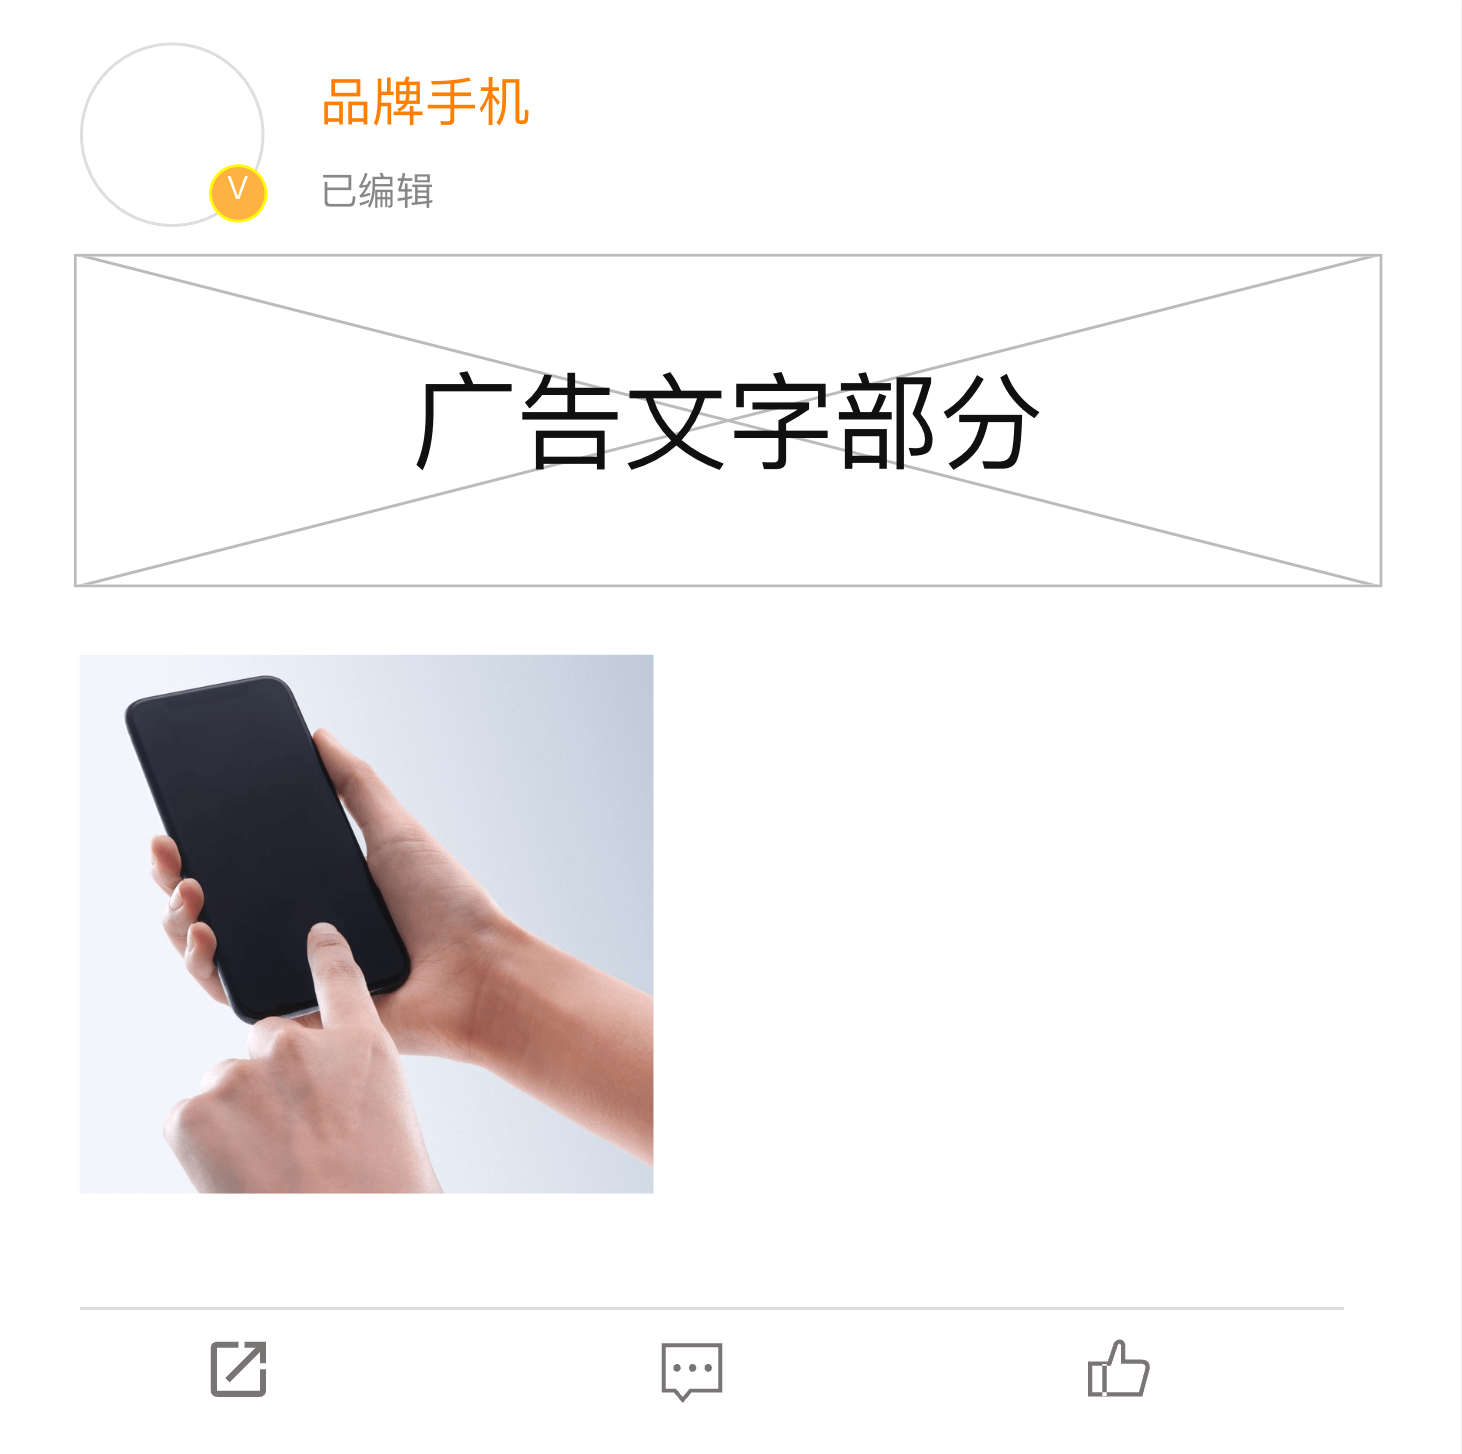
\includegraphics[width=.3\linewidth]{Image/Study2-exp2.png}
    \caption{\label{fig:Study2-exp2-ad-example}实验开始前的广告示意图}
\end{figure}


\subsection{结果}
本实验的分析方法与实验1相似,分别对不同信息创作者(人类专家/AI/AI修改专家)生成的个性化广告效果进行检验。个性化效果通过建立人格水平与因变量(说服效果、微博互动意愿、支付金额)之间的线性回归模型来衡量,其中人格水平作为自变量,三个效果指标作为因变量。由于在本实验中,个性化广告是针对各人格维度的高水平个体进行设计的,因此理论上,当参与者在某一人格维度的得分越高时,相应维度的个性化广告的效果指标应表现更好。此外,由于支付金额的范围较广(0-10000元),在分析过程中对其进行了归一化处理。

结果表明,在三个广告效果指标上,AI (GPT-4) 和 AI 修改专家组 (GPT-4 修改专家) 在宜人性、外倾性、尽责性和开放性四个维度上均表现出稳定且显著的个性化效果(回归显著,\textit{p}s < 0.05)。这说明,特质得分越高,针对高特质设计的广告效果越好,符合预期。而在神经质维度上,三个创作者的广告均表现出稳定的负向结果,即神经质得分越低,针对高神经质设计的广告效果评价越高。人类专家组在外倾性、尽责性和开放性维度上也表现出显著的个性化效果,且与 AI 组和 AI 修改专家组结果一致。但在人类专家组中,宜人性维度的个性化效果不显著(\textit{p} > 0.05)。

\begin{table}[H]
    \centering
    \caption{\label{tab:slope_difference_study2} 不同创作者的回归斜率差异(说服效果)}
    {\tablesongti
    \renewcommand{\arraystretch}{1.2} % 调整行距
    \begin{tabularx}{\linewidth}{>{\centering\arraybackslash}p{3cm} >{\centering\arraybackslash}p{4cm} >{\centering\arraybackslash}p{4cm} >{\centering\arraybackslash}p{4cm}} % 居中对齐
        \toprule
        \textbf{特质} & \textbf{人类专家 (系数 \& }\textit{p}\textbf{ 值)} & \textbf{GPT-4 (系数 \& }\textit{p}\textbf{ 值)} & \textbf{GPT-Loop (系数 \& }\textit{p}\textbf{ 值)} \\ 
        \midrule
        \textbf{外倾性}   & 0.3145 (0.002**)  & 0.3143 (0.001**)  & 0.3431 (0.001**)  \\
        \textbf{宜人性}   & 0.1270 (0.419)  & 0.4350 (0.003**)  & 0.6969 (<0.001***)  \\
        \textbf{尽责性}   & 0.3221 (0.002**)  & 0.4375 (<0.001***)  & 0.4022 (0.001**)  \\
        \textbf{神经质}   & -0.3358 (0.001**)  & -0.3423 (0.001**)  & -0.4036 (0.001**)  \\
        \textbf{开放性}   & 0.4017 (0.004**)  & 0.4859 (<0.001***)  & 0.6110 (<0.001***)  \\
        \bottomrule
    \end{tabularx}
    }
    \caption*{\raggedright \footnotesize 注:*** \textit{p} < 0.001,** \textit{p} < 0.01,* \textit{p} < 0.05,\textsuperscript{\dag} \textit{p} < 0.1。}
\end{table}


进一步,我们比较了三类信息创作者在回归斜率上的显著性差异。结果表明,仅在宜人性维度上,AI 修改专家组与人类专家组在说服效果(\textit{t} = 2.66,\textit{p} = 0.008)和微博互动意愿(\textit{t} = 1.96,\textit{p} = 0.05)两个指标上表现出显著差异。人类专家组本身的个性化效果不显著,而 AI 和 AI 修改专家组的个性化效果显著且稳定。同时,显著性差异检验表明 AI 修改专家组显著优于人类专家组。这一结果说明,GPT-4 在优化人类专家文案时能够显著提升宜人性维度广告的效果。此外,与实验1相比,人类专家组在宜人性维度上的表现发生了变化:实验1中,人类专家组的宜人性个性化效果显著,而本实验中则未达到显著性水平。为探讨这一差异,本研究分析了实验1和本实验所使用的人格测量工具(BFI-10 和 BFI-44)的相关性(如图\ref{fig:study2-correlation})。结果显示,宜人性维度的相关性较低(0.67),而其他四个维度的相关性均较高(>0.80)。这表明,本实验中使用的 BFI-44 测量工具具有更高的精确度和可靠性,因此本实验的结果更可信。此外,在实验1中,人类专家组在外倾性和尽责性维度上未表现出显著的个性化效果,但在本实验中,这两个维度的效果变得更显著。结合测量工具的改进,可以推测,使用更精细的量表后,外倾性和尽责性维度的个性化效果更加稳定。

\begin{figure}[H]
    \centering
    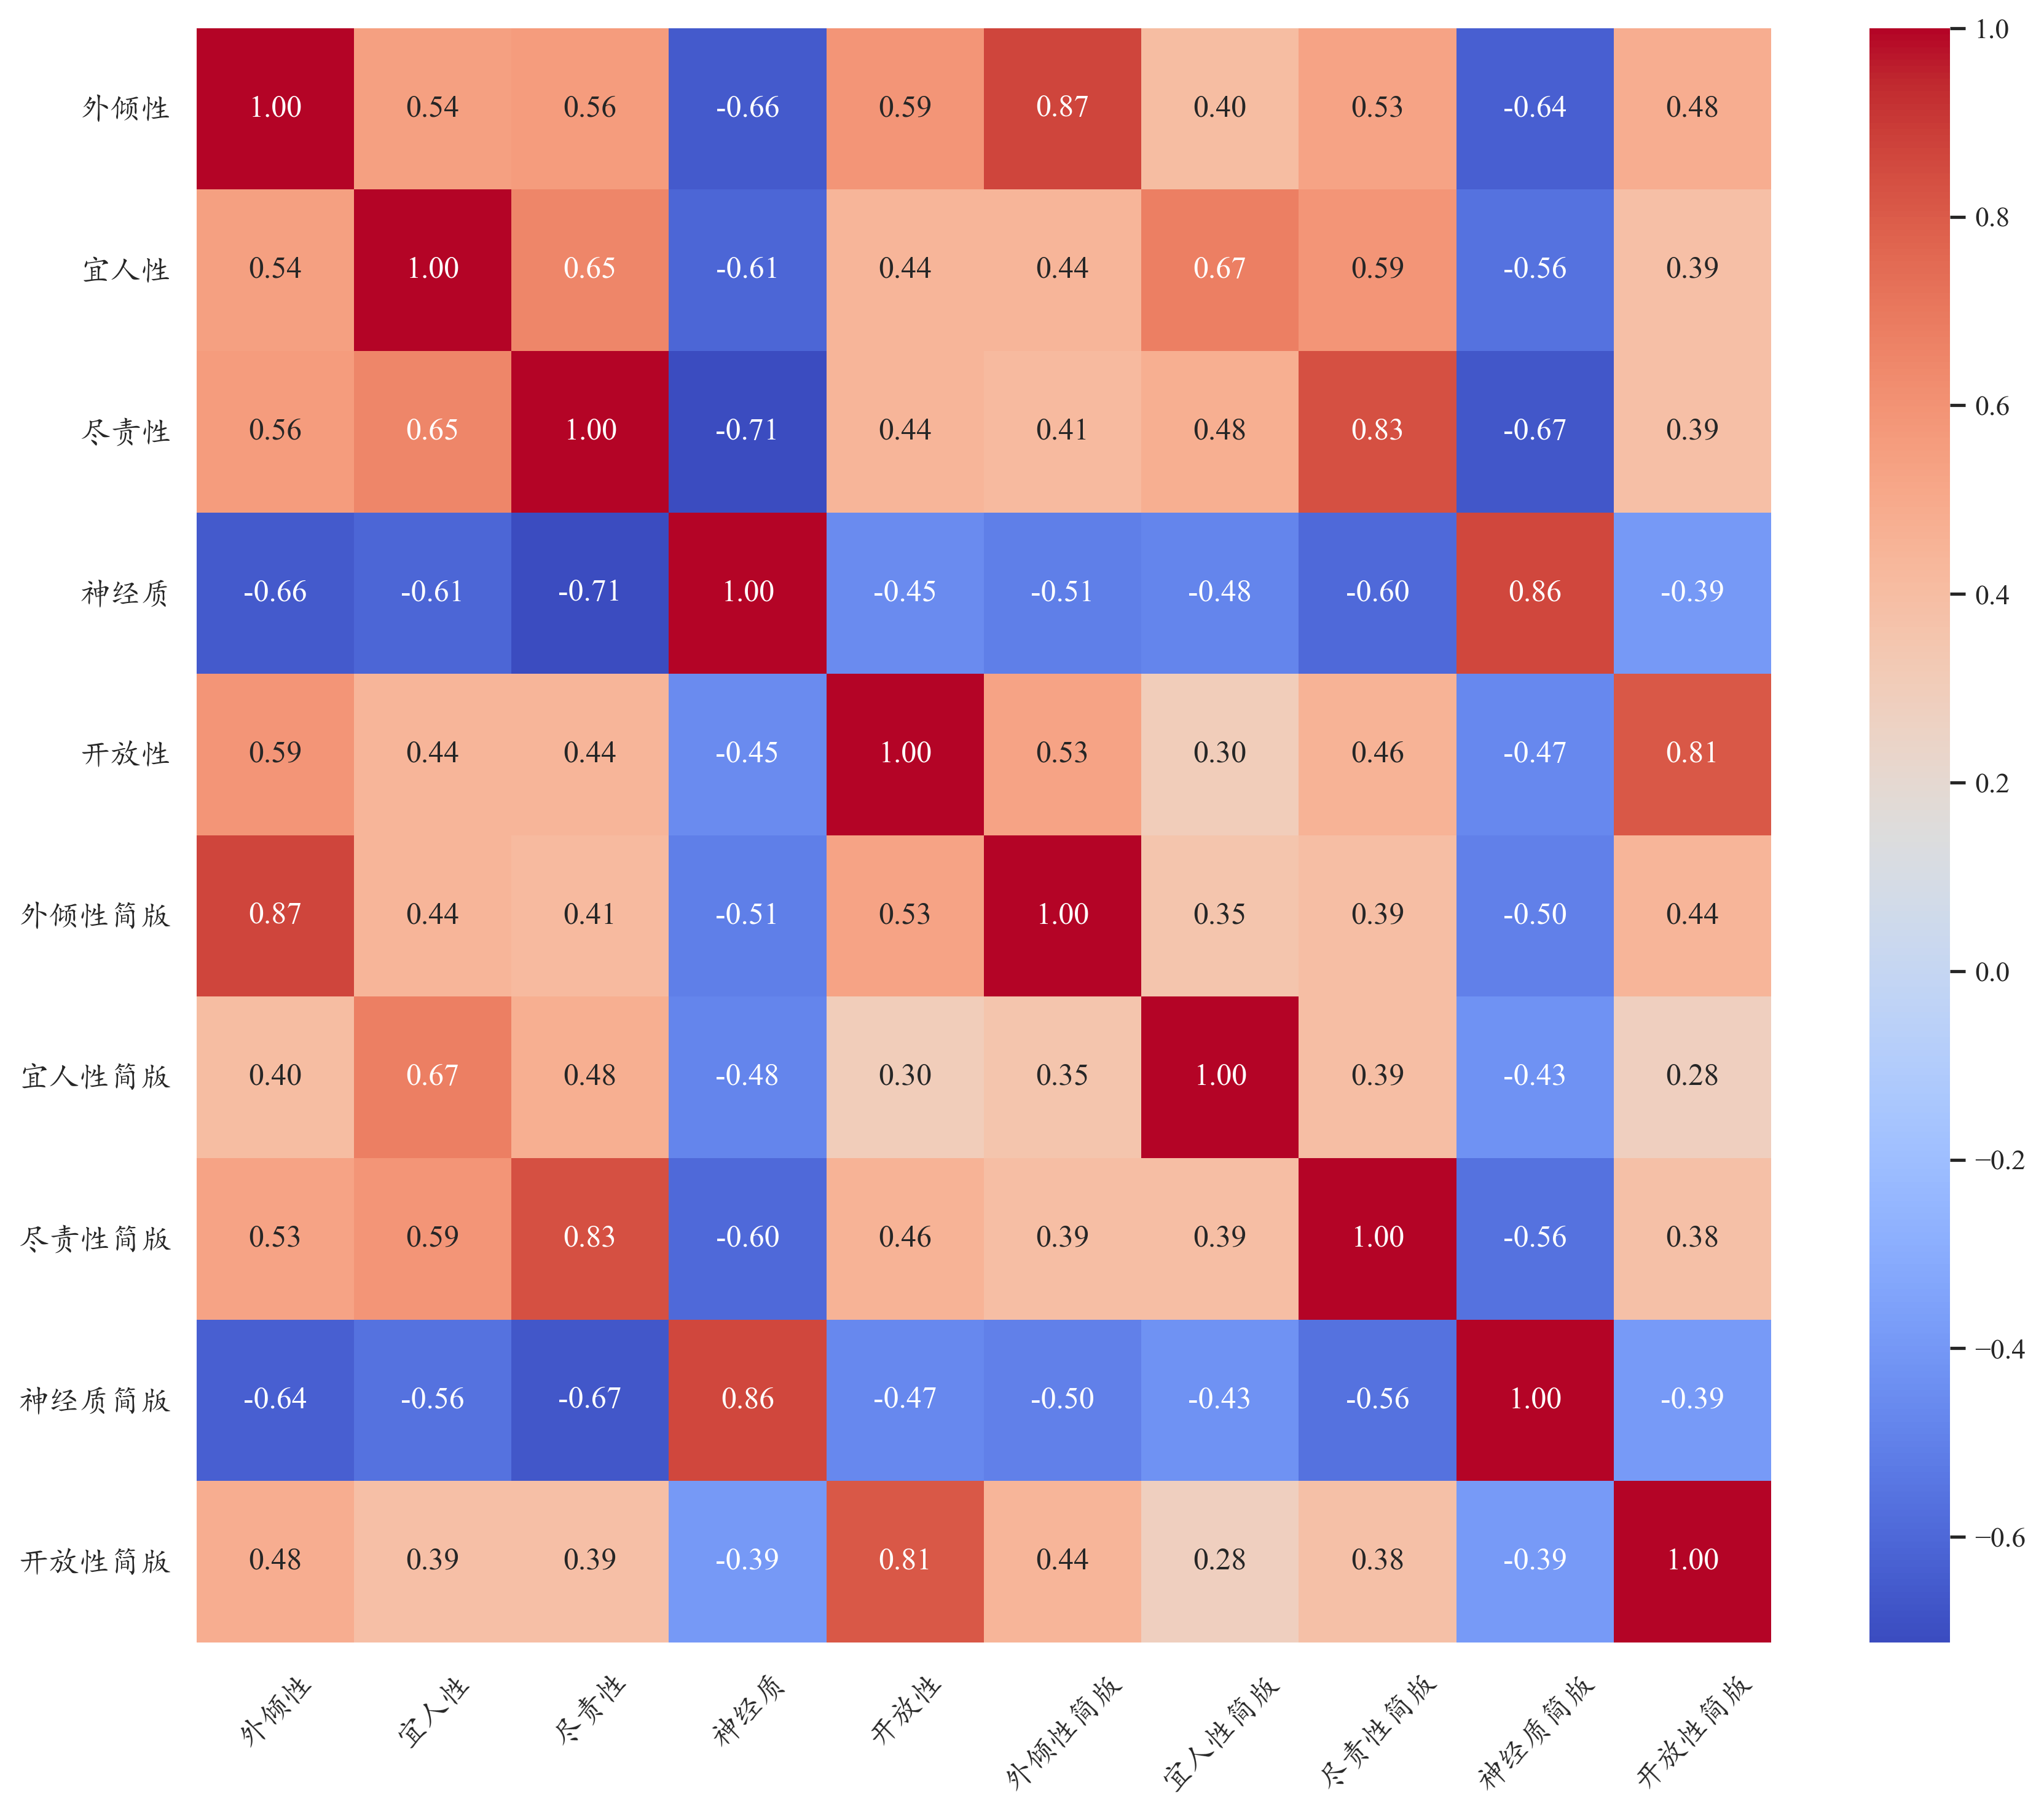
\includegraphics[width=1\linewidth]{Image/BFI44-BFI10相关.png}
    \caption{\label{fig:study2-correlation}BFI44-BFI10相关}
\end{figure}

神经质维度的负向结果表现出一致性。以说服效果为例,AI组(\textit{$\beta$} = -3.410, \textit{p} < 0.01),人类专家组(\textit{$\beta$} = -3.441, \textit{p} < 0.01),AI修改专家组(\textit{$\beta$} = -3.571, \textit{p} < 0.01)在神经质维度上均呈现显著负向预测趋势,即神经质得分较低的个体对针对高神经质设计的广告评价更高。这一结果与前人研究中提到神经质的特殊性一致\citep{matz2024potential}。这一现象的机制可能与高神经质广告传递的情感特征有关,后续研究将进一步结合对 AI 生成广告特征的内容分析进行深入探讨。

综上所述,本实验的结果表明,AI 和 AI 修改专家组在宜人性、外倾性、尽责性和开放性维度上均表现出显著且稳定的个性化效果,而人类专家组在宜人性维度上的表现不如预期,但在外倾性、尽责性和开放性维度上仍显示出一定能力。特别是AI修改专家组在宜人性维度上的显著提升,进一步证明 AI 技术不仅能够独立生成高效的个性化广告,还可以通过与人类专家协作进一步优化广告内容,从而为个性化广告设计中的人机协作提供重要启示。




